\chapter{Evaluation}
% \label{ch:relatedwork}
In order to evaluate the efficiency of our approach, we evaluated it on two real-world applications. These apps 
are on completely different hardware with a completely different framework and different use cases. We will 
present and discuss our results for both of them individually by first explaining the experimental setups involved 
and then provide reasoning for the results obtained. \\

\section{Experimental Setup \textemdash TempSens}
For our first experimental setup, the application we use is called \texttt{TempSens}. It is a mock app that 
was developed from scratch. It continuously monitors and log sensor data from a DHT11 sensor which is used 
to monitor temperature and humidity levels. Overall, 
the app is very simple and has a basic functionality: continuously monitor data and communicate it with the server 
every 60 seconds. The hardware configuration in this setting utilizes a Raspberry Pi 4 Model B running 
a headless Raspbian OS as an edge device where it functions as a client, and a remote server deployed on a MacBook 
Pro running Big Sur. \\
Raspberry Pi 4 Model B houses a System-on-Chip (SoC) which makes it much more affordable and reliable in terms of 
computing capability. It uses BCM2711 as its SoC type which is one of more energy and cost effective alternatives 
than its previous counterparts. The \texttt{TempSensClient} is written in Python 3 and uses RPi.GPIO to interface 
with the sensors. Figure \ref{fig:gpio} shows an extension board that is used to connect sensors to the Raspberry Pi. 
Figure \ref{fig:gpiotable} on the other hand provides the naming methods used for WiringPi, Board and the 
intrinsic pin name for GPIO extension board. For instance, for GPIO27, the WiringPi naming method is 2, Board naming 
method is 13 and its intrinsic name is GPIO2 \cite{gpio}. The overall circuitry resembles that in the figure \ref{fig:circuit}.
WiringPi \cite{wiring} is the CPP library for Raspberry Pi to interact with a GPIO extension board and Board 
\cite{pypi} is a Python library 
for the same purpose. 


\begin{figure}
    \begin{center}
        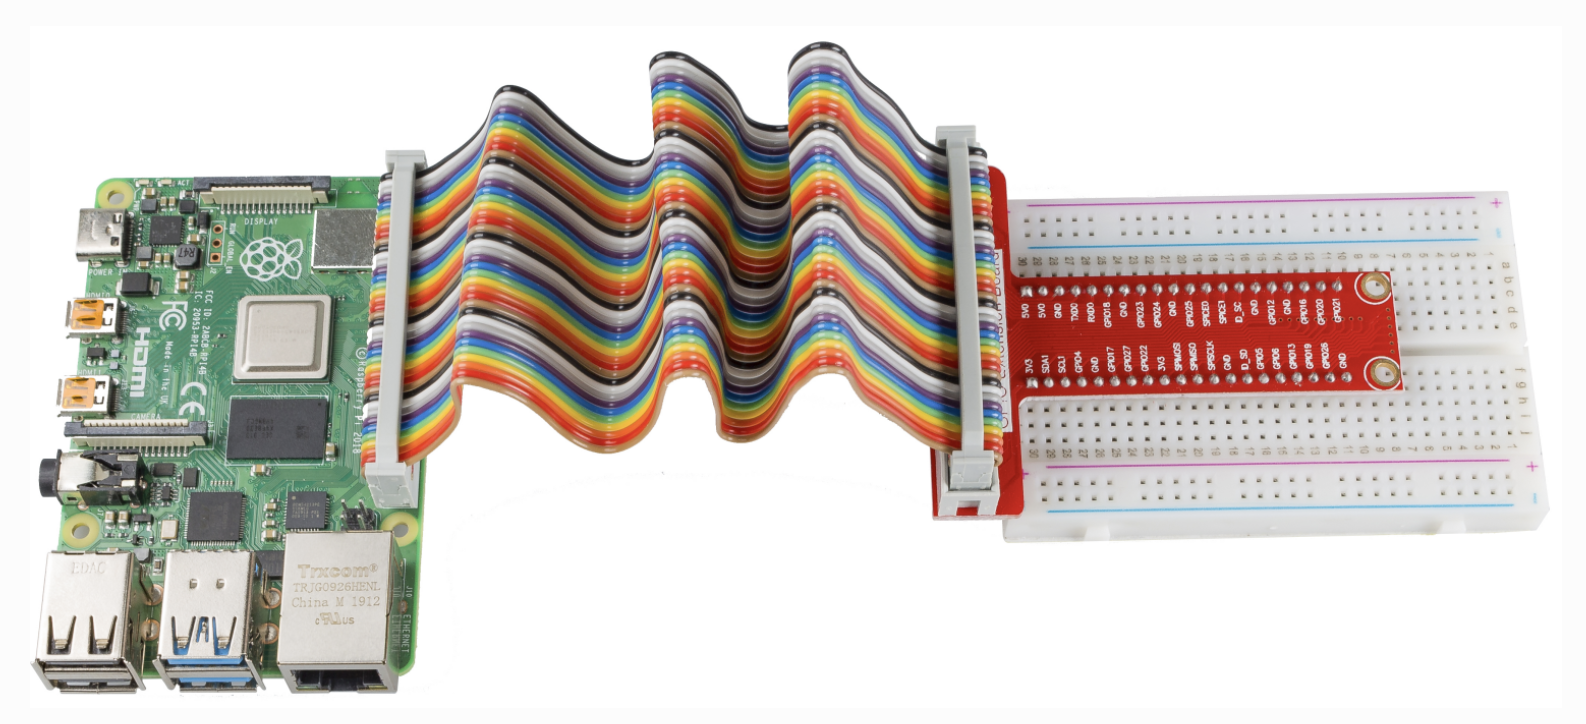
\includegraphics[scale=0.55]{Figs/gpio.png}    
    \end{center}
    \caption{A GPIO extension board \cite{gpio}}
    \label{fig:gpio}
\end{figure}

\begin{figure}
    \begin{center}
        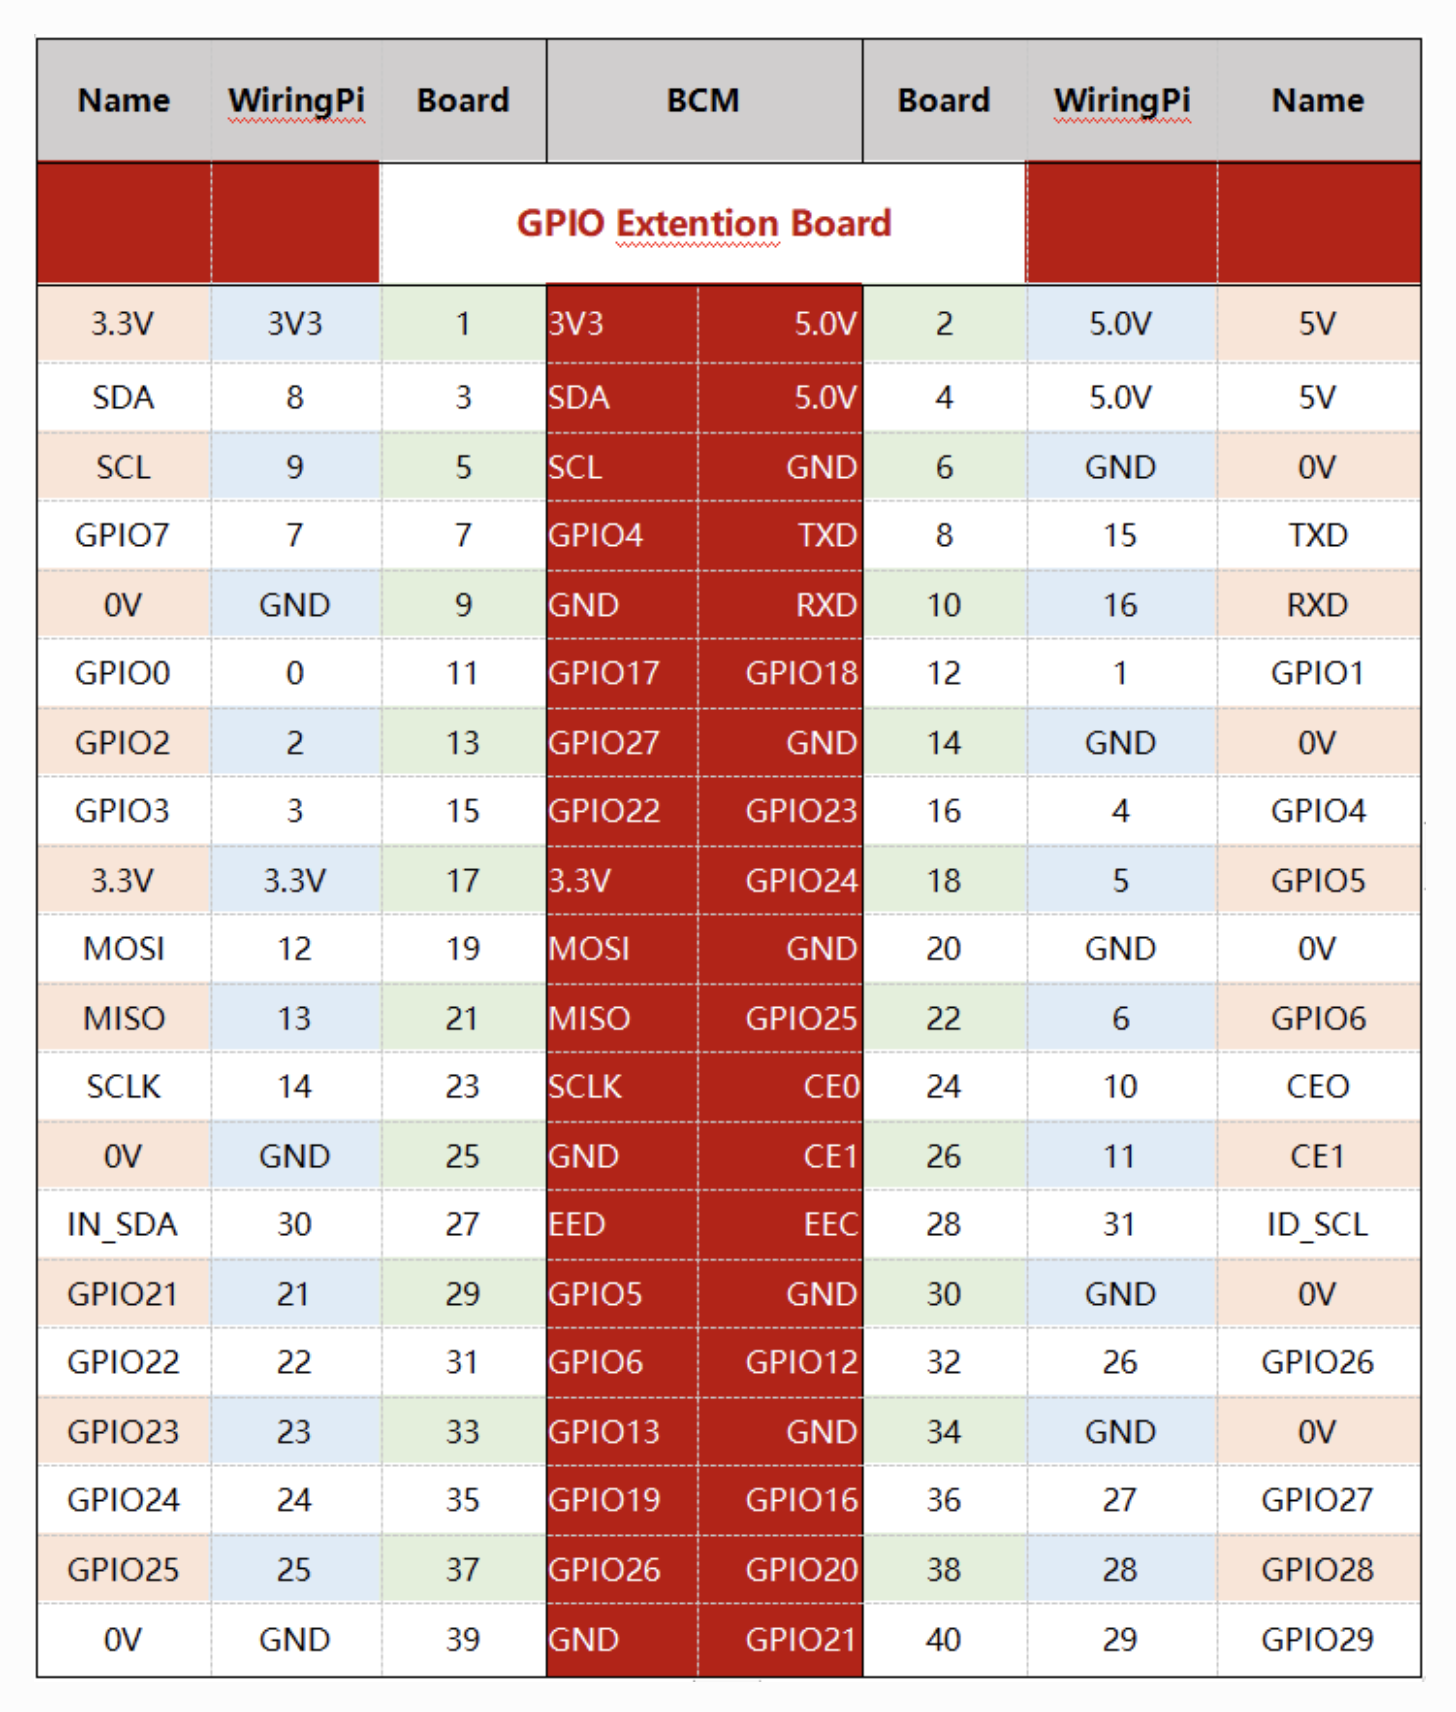
\includegraphics[scale=0.45]{Figs/gpiotable.png}    
    \end{center}
    \caption{Naming methods for WiringPi and Board \cite{gpio}}
    \label{fig:gpiotable}
\end{figure}

\begin{figure}
    \begin{center}
        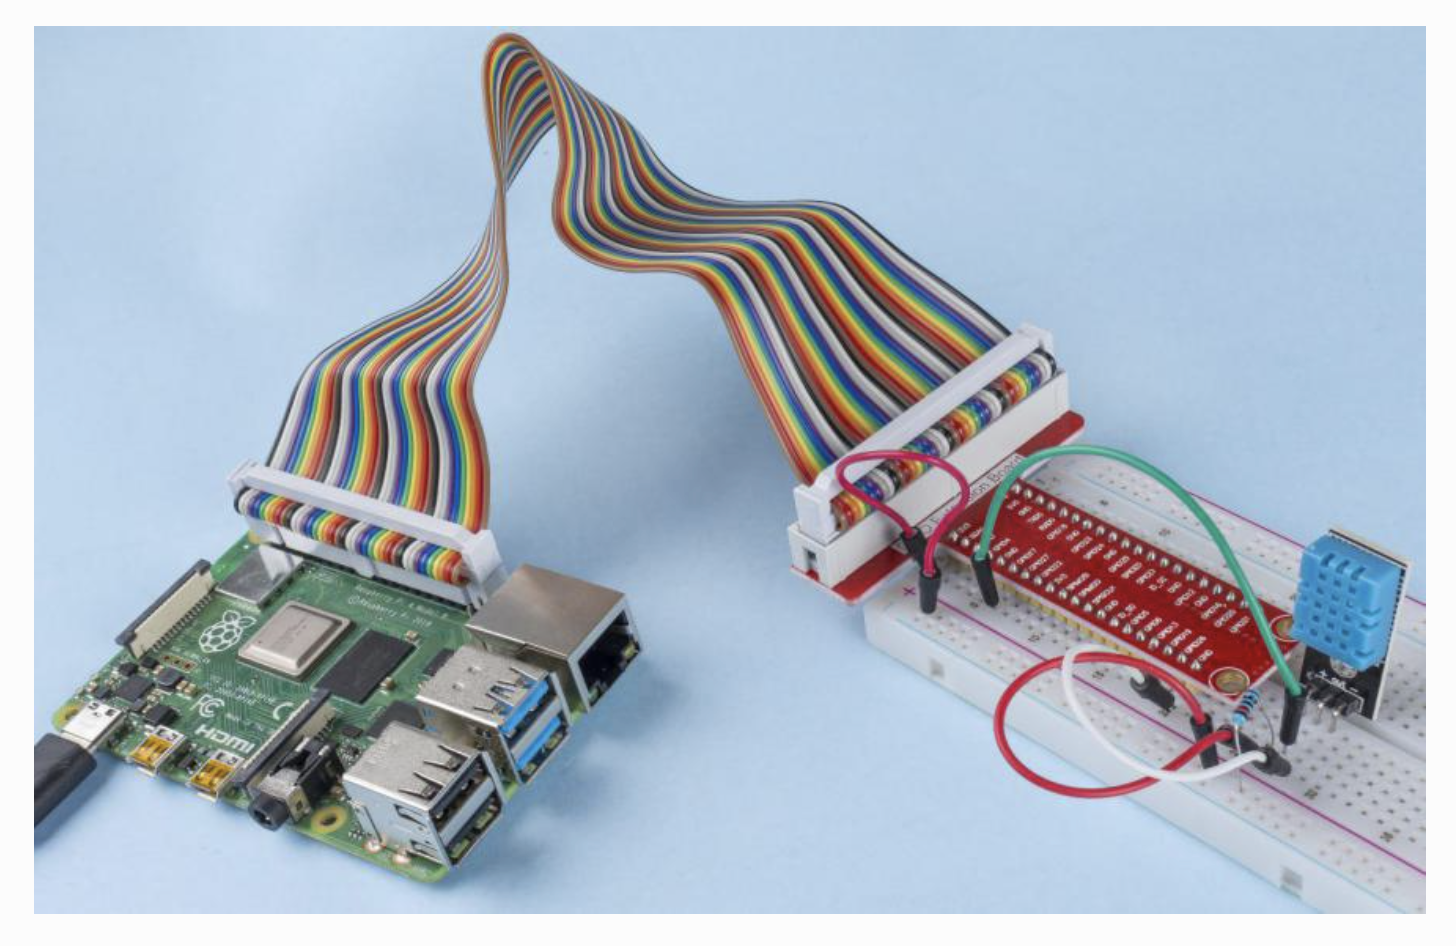
\includegraphics[scale=0.45]{Figs/circuit.png}    
    \end{center}
    \caption{TempSens Hardware Configuration  \cite{circuit}}
    \label{fig:circuit}
\end{figure}

The communication is done over TCP/IP with the help of socket programming. The \texttt{TempSensServer} 
is a bare-bone server which just displays the received information in a proper format. The client collects data for 
one minute before sending the accumulated data to the server. By default, it uses 512 bytes as chunk size. \\
Based off figure \ref{fig:bcm}, the estimated power consumption of wifi adapter is \texttt{1.542} Watts. This 
is calculated after computing the mean average sum of different power modes for different current values 
corresponding to the voltage. In order to compute the optimal chunk size, the python script to determine the 
chunk size was run on the Raspberry Pi 4. \\

\begin{figure}
    \begin{center}
        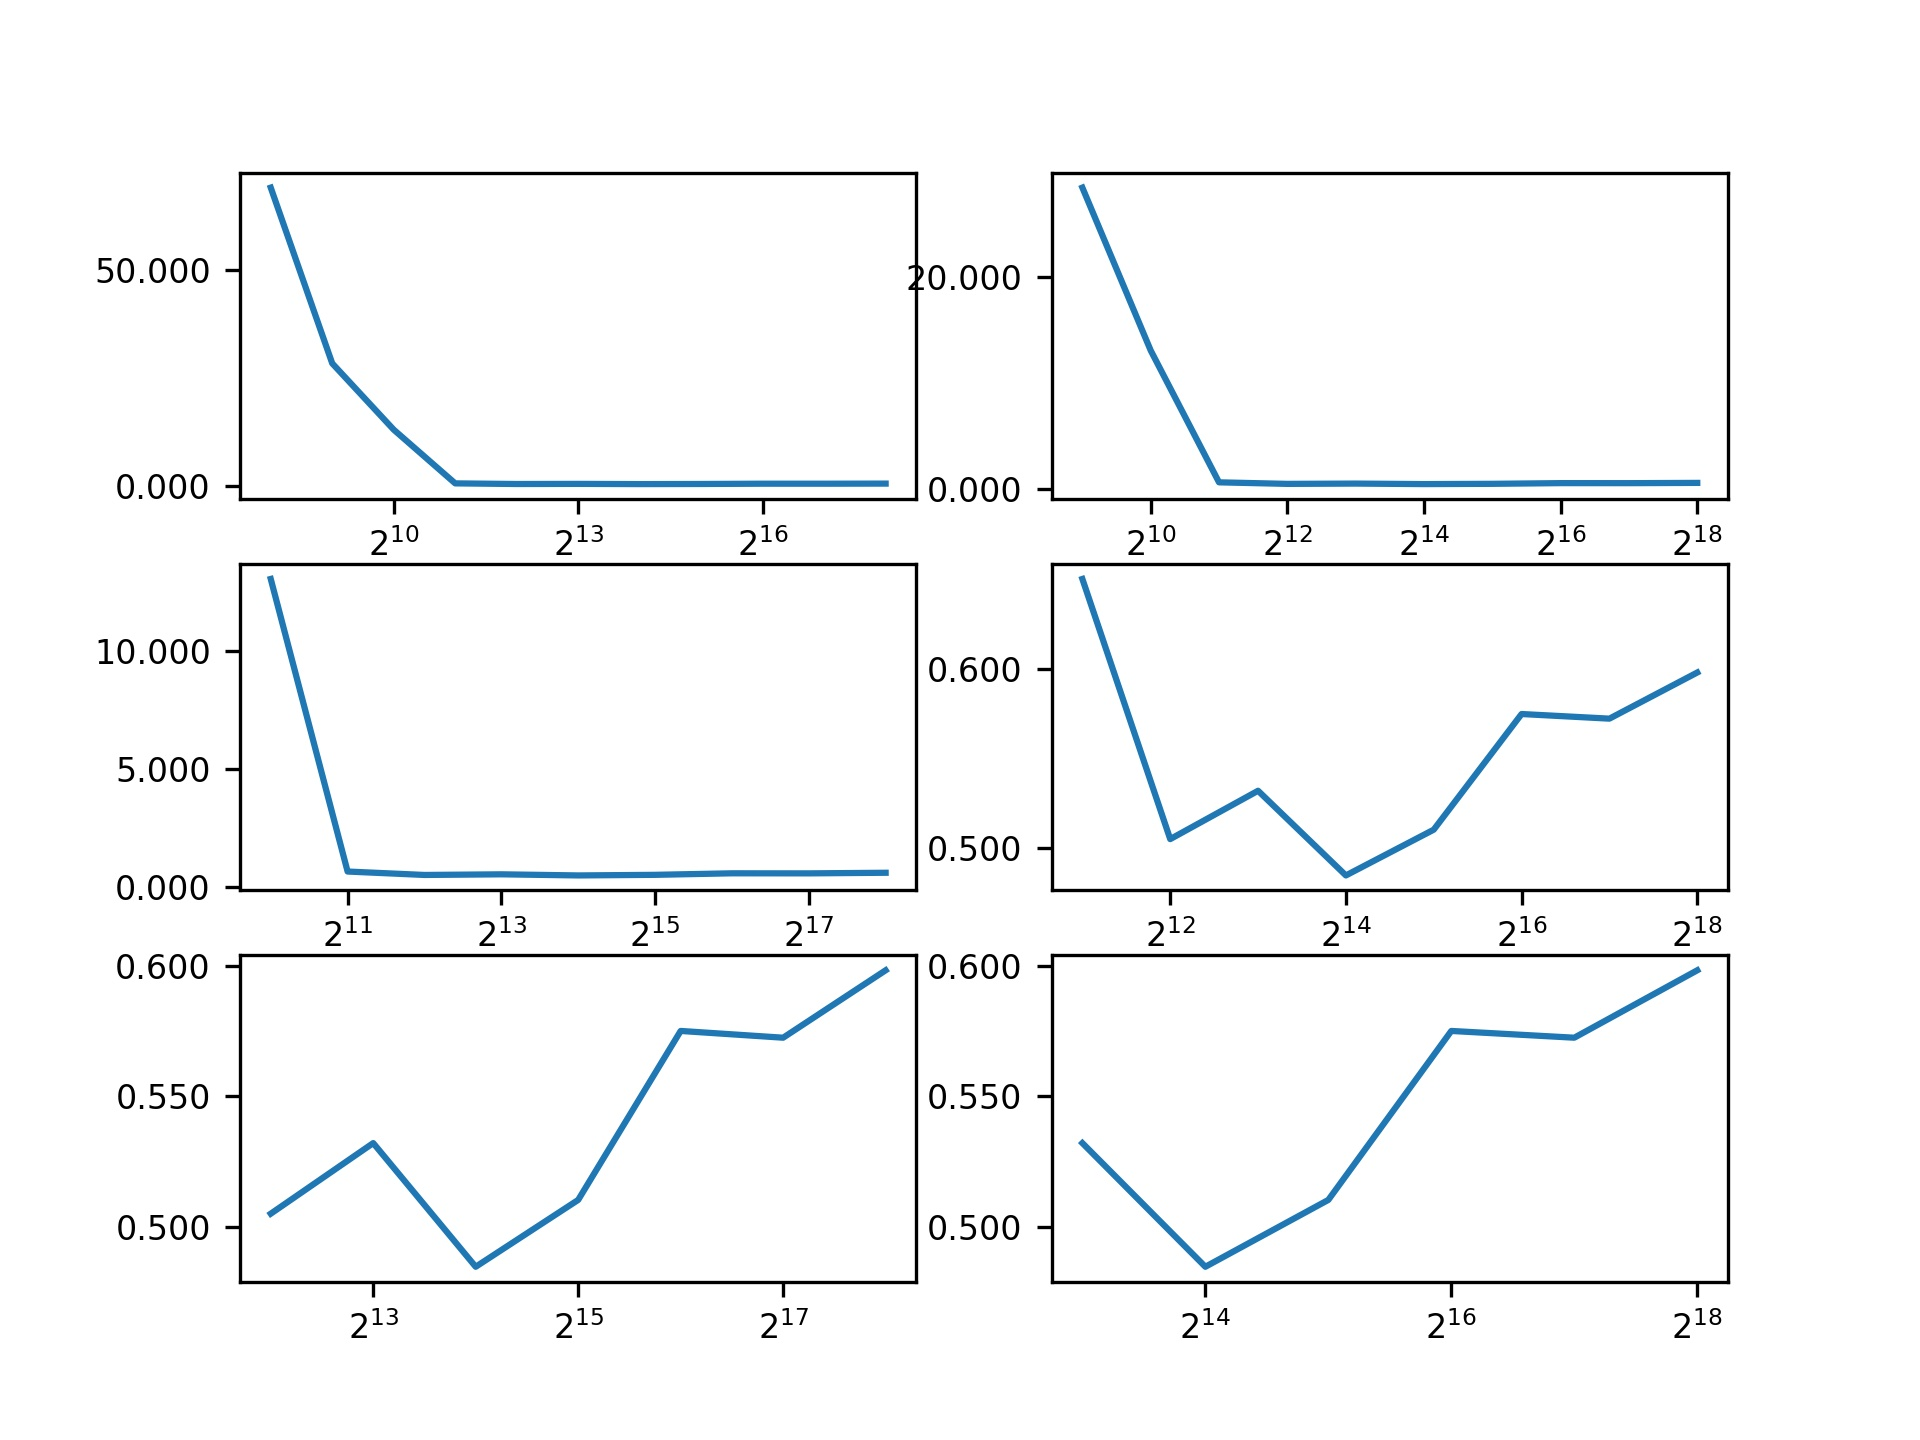
\includegraphics[scale=0.23]{Figs/epbpi.png}    
    \end{center}
    \caption{EPB for different chunk sizes (Chunk Size (x-axis) and Energy in microJ (y-axis))}
    \label{fig:epbpi}
\end{figure}

Figure \ref{fig:epbpi} shows that energy consumption does not linearly depend on chunk size. If that were the case, 
we would have got a straight line. However, what we observe is a global minima and around \texttt{$2^{14}$} on 
the x-axis, we see that's where the lowest amount of energy is being consumed per byte. This suggests that 
for the \texttt{TempSens} app to have optimal energy consumption for communication, the preferred chunk size 
should be \texttt{$2^{14}$} as it would consume the lowest amount of energy. It can also be seen that EPB at \texttt{$2^{14}$} 
is significantly lower than that at the initial value of \texttt{$2^{8}$}. Figure \ref{fig:epbpi} shows multiple 
subplots each for a different range of chunk sizes. The idea behind this is to show that even though the energy 
usage looks pretty much the same when seen in the top-left and top-right plot, but when you actually zoom in 
and see the bottom-left and bottom-right plots, you realize that the energy usage is not that linear anymore. 
There's clearly a global minima present and it will be different for different devices due to varying 
hardware and software configuration but with our work we can definitely find it. \\
Based on the values obtained from this experiment, and then replace them with the default values in \texttt{TempSensClient}, 
the total amount of time for which battery life was prolonged solely due to saving energy in communication cost. 
was about 3 minutes. However, one other use-case of this approach is to be able to determine the intervals at 
which one should communicate data, if it allows. In the case of \texttt{TempSens}, its quite flexible as 
the information being communicated is not time sensitive and the use-case is not that critical. This suggests that 
an optimal interval would be just when the app collects enough amount of data (\texttt{$2^{14}$}). For this app, 
it turned out to be 120 seconds which is double the original interval break. Applying this optimization, we were 
able to prolong the battery time of one charge cycle by 7 minutes. Even though apparently it doesn't sound like much 
but keep in mind this is just with optimizing communication cost which is usually in terms of microJoules. 
Comparatively, that is a considerable improvement in the overall scheme of things. On the other hand, it would 
not have mattered much if the energy usage of the whole device was dependent on a sensor which consumes 
much more energy as compared to the wifi adapter as we will discuss it in the next experimental setup. \\

\section{Experimental Setup \textemdash Fall Detection App}
For this experiment, we test our approach on the Fall Detection App \cite{falld}.
